Encuentra el valor de la incógnita en el triángulo de la figura \ref{fig:angle_triangle_31}.

\begin{minipage}[t][5.5cm][b]{0.3\textwidth}
    \begin{figure}[H]
        \centering
        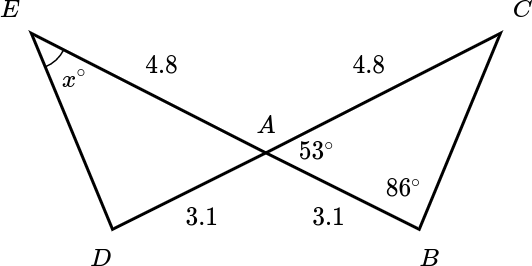
\includegraphics[width=1\linewidth]{../images/angle_triangle_31.png}
        \caption{}
        \label{fig:angle_triangle_31}
    \end{figure}
\end{minipage}\hfill
\begin{minipage}[t]{0.65\textwidth}
    \begin{solutionbox}{5.5cm}
        $\angle DAE$ forma un ángulo opuesto por el vértice con $\angle BAC$.
        \[\Rightarrow \angle DAE = \angle BAC \]
        $\triangle ABC$ y $\triangle ADE$ también tienen dos lados iguales.
        \[\therefore \triangle ABC \cong \triangle ADE\]
        Los triángulos congruentes también tienen ángulos congruentes (iguales).
        Observamos que el ángulo $x$ corresponde al $\angle ACB$ y
        $\angle ACB$ mide:
        \[x=180^\circ-53^\circ-86^\circ=41^\circ\]
    \end{solutionbox}
\end{minipage}
